\tikzstyle{module}=[black, rectangle, rounded corners, fill=blue!20, minimum height=6mm, draw]
\tikzstyle{depend}=[black, thick, ->, >=stealth]
\tikzstyle{optional}=[black, thick, dashed, ->, >=stealth]
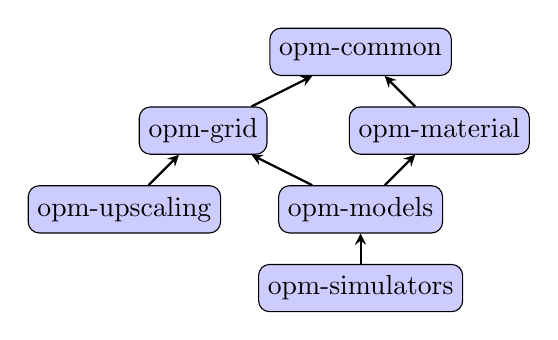
\begin{tikzpicture}[scale=1.0]

  \node [module] (opm-common) at (5,4) {\Code{opm-common}};
  \node [module] (opm-material) at (6,3) {\Code{opm-material}};
  \node [module] (opm-grid) at (3,3) {\Code{opm-grid}};
  \node [module] (opm-upscaling) at (2,2) {\Code{opm-upscaling}};
  \node [module] (opm-models) at (5, 2) {\Code{opm-models}};
  \node [module] (opm-simulators) at (5,1) {\Code{opm-simulators}};

  \draw [depend] (opm-material) to (opm-common);
  \draw [depend] (opm-grid) to (opm-common);
  \draw [depend] (opm-models) to (opm-material);
  \draw [depend] (opm-models) to (opm-grid);
  \draw [depend] (opm-upscaling) to (opm-grid);
  \draw [depend] (opm-simulators) to (opm-models);

\end{tikzpicture}


